% !Mode:: "TeX:DE:UTF-8:Main"

\documentclass[aspectratio=169]{beamer}
\usepackage{tikz}
\usetikzlibrary{tikzlings}
\usetikzlibrary{decorations.text,fpu}
\usepackage{xkcdcolors}
\usepackage[svgnames,x11names]{xcolor}

\setbeamertemplate{navigation symbols}{}

% trick taken from https://topanswers.xyz/tex?q=1989
\tikzset{
    use page relative coordinates/.style={
        shift={(current page.south west)},
        x={(current page.south east)},
        y={(current page.north west)}
    },
 }

\makeatletter
\newcommand*{\slideinframe}{\number\beamer@slideinframe}
\makeatother
\newcommand\bobblehat[2]{%
  \begin{scope}[shift={(-0.68,3)},scale=0.006,yscale=-1]
\begin{scope}[yshift=-100]
  \path[fill=#1] (47.9231,182.0769) -- (45.0000,179.1539) -- (45.0000,162.5000)
  -- (45.0000,145.8461) -- (47.9453,142.9008) -- (50.8907,139.9555) --
  (112.9180,140.2277) -- (174.9453,140.5000) -- (177.2227,142.7751) .. controls
  (179.3851,144.9355) and (179.5159,145.9071) .. (179.8160,162.0361) --
  (180.1320,179.0219) -- (177.1429,182.0109) -- (174.1539,185.0000) --
  (112.5000,185.0000) -- (50.8462,185.0000) -- cycle;
\end{scope}
\path[fill=#2]  (56.5667,132.7500) ..
  controls (59.5944,107.7429) and (75.2960,83.7816) .. (94.5000,74.8622) ..
  controls (97.2500,73.5849) and (99.6847,72.4212) .. (99.9105,72.2761) ..
  controls (100.1363,72.1310) and (99.4613,71.0322) .. (98.4105,69.8342) ..
  controls (97.3597,68.6363) and (97.0114,67.9536) .. (97.6365,68.3170) ..
  controls (98.2616,68.6804) and (97.9849,67.4318) .. (97.0216,65.5423) ..
  controls (95.4197,62.4003) and (95.3072,60.1643) .. (96.3771,52.7307) ..
  controls (96.6846,50.5944) and (104.0082,42.8871) .. (105.0934,43.5577) ..
  controls (105.5160,43.8189) and (106.1490,43.5679) .. (106.5000,43.0000) ..
  controls (106.8510,42.4321) and (107.5193,42.2029) .. (107.9852,42.4908) ..
  controls (108.4510,42.7787) and (109.9790,42.5783) .. (111.3807,42.0454) ..
  controls (113.0425,41.4136) and (114.1417,41.4203) .. (114.5400,42.0647) ..
  controls (114.8759,42.6083) and (115.6794,42.9689) .. (116.3254,42.8662) ..
  controls (118.5731,42.5085) and (122.5221,44.8299) .. (126.0000,48.5533) ..
  controls (127.9250,50.6142) and (128.9426,51.9844) .. (128.2614,51.5982) ..
  controls (127.4296,51.1267) and (127.2185,51.4058) .. (127.6184,52.4481) ..
  controls (127.9460,53.3016) and (128.5244,54.0000) .. (128.9039,54.0000) ..
  controls (129.8323,54.0000) and (129.6284,61.1769) .. (128.6553,62.7500) ..
  controls (128.2299,63.4375) and (128.1853,64.0000) .. (128.5560,64.0000) ..
  controls (128.9267,64.0000) and (128.4566,65.1804) .. (127.5113,66.6231) ..
  controls (126.3361,68.4167) and (126.2206,69.0251) .. (127.1462,68.5469) ..
  controls (127.8908,68.1623) and (127.4817,68.7463) .. (126.2370,69.8446) --
  (123.9741,71.8415) -- (129.6984,74.4622) .. controls (149.5630,83.5565) and
  (165.3543,107.3191) .. (168.4332,132.7500) -- (169.0689,138.0000) --
  (112.5000,138.0000) -- (55.9311,138.0000) -- (56.5667,132.7500) -- cycle;

\end{scope}}
\newcommand\candlescalefactor{3}

\tikzset{%
 lines/.style={
    ultra thick,
    line join=round,
    line cap=round
  }, sketch/.style={
    bend right, out=rand*10, in=180-rand*10
  }}
  
\ExplSyntaxOn
\let\intmodnn\int_mod:nn
\ExplSyntaxOff

     
\begin{document}

\def\steps{50}
\begin{frame}
  \begin{tikzpicture}[
     %use page relative coordinates,     
      remember picture,
      overlay
    ]
      \node[anchor=north,inner sep=0pt] at (current page.north) 
      {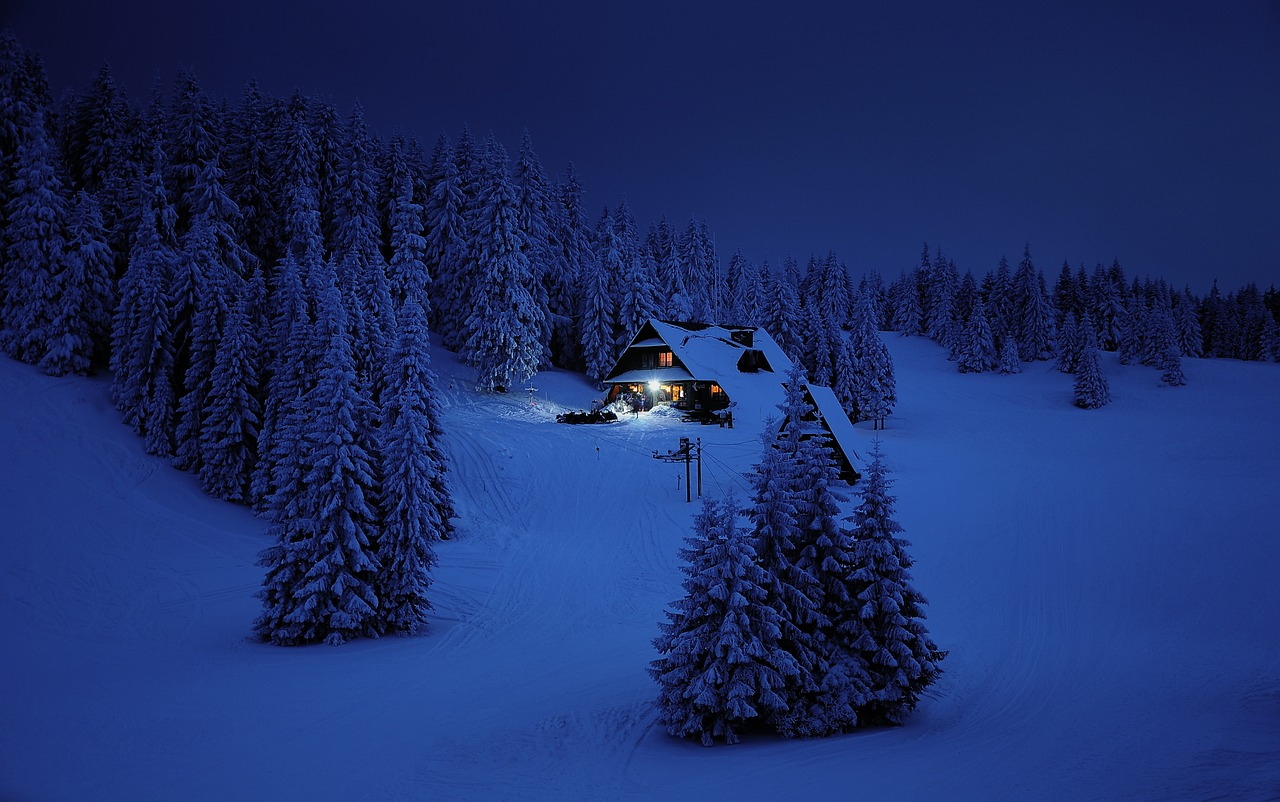
\includegraphics[width=\paperwidth]{snow}}; 
   
 \node[white,text width=\paperwidth,font=\tiny,align=center] at ([yshift=-0.25cm]current page.north) {https://pixabay.com/de/photos/schnee-winter-berge-haus-heimat-3373432/};        
    
  \end{tikzpicture}  
  %\pause[\steps]
 
\vfill  \hspace*{\fill}\begin{tikzpicture} 

\path[use as bounding box](-2cm,1cm) rectangle (0.5cm,2cm); 

\node[inner sep=0pt]{ 
		\ifnum \intmodnn{\thepage}{6} > 2
			%
\includegraphics[width=3cm]{mouse_close}%
		\else
			%
\includegraphics[width=3cm]{mouse_open}%
		\fi%
	};
 \begin{scope}[scale=1.3,xshift=-0.49cm,yshift=-1.3cm]\bobblehat{xkcdCloudyBlue}{xkcdDullBlue} \end{scope} 

 \begin{scope}[scale=1/\candlescalefactor,xshift=-0.2cm,yshift=-3cm]
\pgfmathsetseed{10} 
%\foreach \n in {1,...,10}{ 
%  \tikzset{xshift=\fpeval{\candlescalefactor*(\n-0.8)/\duckscolumns}\textwidth}%
  \fill [lines, fill=Red1, rounded corners=0.125cm]
    (-1/3,0) to [sketch] (-1/3,2) -- (1/3,2)  to [sketch] (1/3,0);
%    }
\pgfmathsetseed{\slideinframe}
% \foreach \n in {1,...,10}{
%  \tikzset{xshift=\fpeval{\candlescalefactor*(\n-0.8)/\duckscolumns}\textwidth}%
  % Wick
  \draw [lines] (0,2) -- ++(0,1/4);
  \tikzset{shift={(0,2+1/8)}, xscale=round(rnd)*2-1,yscale=1+rand/8}
  \foreach \s/\c in {1/yellow,.5/red}
    \path [lines, fill=\c!50!orange, scale=\s]
      (0,0)
      arc (270:180:3/8)
      .. controls ++(0,1/4) and ++(0,-1/4) .. (0,3/2)
      arc (90:0:3/8 and 1) arc (360:270:3/8 and 1/2);
 %  }
\end{scope}
\end{tikzpicture}
\pause[\steps]    
\end{frame}


\end{document}

\begin{scope}
  \path[clip]
  \duckpathjacket;
  \node[anchor=south west] at (0,0){
\includegraphics[width=3cm]{tartan3}};
 \end{scope}

